\documentclass[conference]{IEEEtran}

\ifCLASSINFOpdf
   \usepackage[pdftex]{graphicx}
   \graphicspath{{../pdf/}{../jpeg/}}
   \DeclareGraphicsExtensions{.pdf,.jpeg,.png}
\else
\fi

% correct bad hyphenation here
\hyphenation{op-tical net-works semi-conduc-tor}

% CUSTOM PACKAGES
\usepackage{amsmath}
\renewcommand{\arraystretch}{1.3}
\usepackage{etoolbox}
\apptocmd{\thebibliography}{\setlength{\itemsep}{0.6pt}}{}{}
\usepackage{url}
\usepackage{caption}
\usepackage{subcaption}
\usepackage{colortbl}
\usepackage{xcolor}
\definecolor{light-gray}{gray}{0.78}
\usepackage{epstopdf}
\usepackage{lettrine}


\begin{document}

\title{A Tool-chain for Instruction Set Architecture Design}

\author{
\IEEEauthorblockN{Alessandro de Gennaro}
\IEEEauthorblockA{School of Electrical and\\Electronic Engineering\\
Newcastle University\\
Newcastle upon Tyne, United Kingdom\\
Email: a.de-gennaro@ncl.ac.uk}
\and
\IEEEauthorblockN{Paulius Stankaitis}
\IEEEauthorblockA{School of Computing Science\\
Newcastle University\\
Newcastle upon Tyne, United Kingdom\\
Email: paulius.stankaitis@ncl.ac.uk}}

\maketitle

\begin{abstract}
Adopting a systematic approach for the design of a processor instruction set is
instrumental for tackling the complexity, which rules most of modern processors.

We present a tool-chain which follows the designer through all the phases of the
design, from the specification of instructions to the hardware synthesis of a
microcontroller. The flow is also meant to simplify the understanding of the
Instruction Set Architecture (ISA) reference manuals. Often, these documents are
semi-formal, hard to read and fully understand. We believe that designers will
benefit from a visual graph-based model, automatically derived from the ISA
specification, and customisable to fit different needs. Some of the tools have
already been developed and tested on ARMv6-M architecture, others yet need to be
fully implemented.

The design flow will be integrated inside the Workcraft framework. We also compare
the presented approach with the others available in the literature.
\end{abstract}

\IEEEpeerreviewmaketitle


\section{Introduction}
\label{sec:intro}
Technology progress allows industries to integrate always more transistors over the
same amount of area, following Moore's law. In turn, design complexity of these
systems progressively increases. This led research to be focused on raising the
level of abstraction of the languages used at the early-stages of design. This work
presents a design flow for an easier specification, visualisation, simulation,
customisation and hardware synthesis of instruction sets.

The consultation of an ISA reference manual (i.e. ARMv6-M \cite{armManual}) can be
a difficult and tedious operation. Anthony Fox, in his attempt to describe a model
of the ARMv7 instruction set, argues: ``official reference manuals are large,
stretching to many hundreds of pages - one can easily overlook subtle details or
become bogged down with ``uninteresting'' background information'' (\cite{armv7},
section 1). And yet: ``official descriptions are semi-formal (ambiguous)''
(\cite{armv7}, section 1). 

In the light of the above, a simple and formal way to specify and, more
specifically, visualise instruction sets is needed. A visual graph-based model can
help designers for a quicker comprehension of the processor. ISAs in fact provide a
software level description of the hardware itself. We use Conditional Partial Order
Graph (CPOG) \cite{cpog},\cite{andreyPhd} as the visualisation model. They can
efficiently represent concurrent and sequential behaviours, and already come with a
tested tool-kit for the customisation, encoding and hardware synthesis
(\cite{workcraft}, \cite{satEncoding}, \cite{acsd}).

We propose a new domain-specific language for ISA specification. The current
implementation is embedded in \textit{Haskell} This is a recent and extremely
flexible functional language, and provides predefined constructs and classes for
our purpose (i.e. monad class).

The article is organised as follows: Section \ref{sec:dsl} describes the framework
we have developed, and how this can be used to interact with all the steps of the 
design flow. Section \ref{sec:arm} presents a case-study: the ARMv6-M ISA. 
And finally, Section \ref{sec:conclusion} summarises the achieved results, 
outlining the future research directions.

\subsection{Related work}

An attempt to use partial orders to describe the instructions of a complex hardware
structure can be found in \cite{maxPhd}. The author uses Conditional Partial Order
Graphs to visually describe the instructions of the Intel 8051 Microcontroller.
Yet, he used them for building an asynchronous controller and managing the internal
execution flow of the datapath elements. The manual construction of partial orders
is an error-prone process. Connecting all the operations taking into account their
dependencies and order is a complex task. This further inspired our research, and
led us to bridge this gap with an automated approach.

Regarding the language we chose to adopt, it is not difficult to find other cases
where functional languages have been used as a starting point for ISA
specification. In this direction, \cite{isaFunc} provides an interesting attempt to
build an infrastructure for instruction set development. The authors developed the
concepts of \textit{state} and \textit{transformations}. The former represents the
current state of the machine, which evolves over time according to the
transformations (instructions). \textit{F. Yuan and K. I. Eder} instead, created a
formal and hierarchical model, which can be refined for fitting the needs of a
particular ISA. This model (characterised in \cite{isaEventB}) is composed by 4
abstract layers. Each of these layers describes a particular aspect of the
instruction set. The deeper the designer explores this hierarchical representation,
the more refined will be the final system.

Another example can be found in \cite{armv7}. The authors here built a framework
which can be extended to tailor instruction sets. They use a monadic programming
style, based on three basic operations: \textit{return}, \textit{bind} and
\textit{parallel}. These are meant to mimic the flow of an entity (the hardware
system), which is always returned as a result of the execution of an instruction.
Instructions can be bound together either sequentially or in parallel. Here, the
case study used is the ARMv7, a widespread instruction set embedded by the 
Cortex-A8 processor. An additional example of how an ISA might be specified inside
a tool is present in \cite{isaXml}. Both the modules and the instructions here are
introduced via a xml-based language, fairly readable but not very flexible.

%------------------------------------------------

% Alex
\section{Domain Specific Language}
\label{sec:dsl}
% DSL introduction
The language used to describe the framework is Haskell \cite{haskell}. This is a 
functional language which fits well to our needs for the high capability to be abstract.
We followed the path, already explored in \cite{armv7}, implementing the \textit{monad class}
to build the infrastructure of the domain specific language (DSL).

The processor is seen as an entity composed by a combination of an internal and
external storage. Respectively, the former is represented by a set of registers,
while the latter by a memory that contains both instructions and data; according to von
Newumann architecture. 

Instructions can be executed by the processor. They are able to modify the current 
state of the modelled machine.

$$P(Regs, Mem) \Rightarrow P'(Regs, Mem)$$

\noindent Every time the processor pulls off an instruction indeed, the state of the machine
evolves into a new state $P'$ different from the previous one. Where either the registers and
the memory might be different. This approach is relatively similar to the one used in
\cite{isaFunc} to describe a processor. We are confident therefore that the high degree of
abstraction which we have attempted to keep will allow us to bidirectionally connect these
two representations.

% Alex
\subsection{Scalability of the framework}
% Description of the microprogram file
%  - how could be extended to fit the microprocessor model
%  - basic functions which each processor implements
%  - types used (Register - ComputationType - Address/Value)
%  - Monad class
%  - Processor seen as a Memory/register entity which evolves over time
What marks our approach is the high degree of flexibility and abstraction that can
extensively tailor every processor. The framework we present in this document is composed
by different layers (modelled in various and interconnected files), each of them plays 
an important and different role in the structure.

The component in charge of modelling the low-level hardware functions is named
\textit{basics}. This is at very bottom layer, close to the hardware.
In this, some of the methods which are used by the processor are implemented: 
reading and writing from/into a memory location; reading
and writing from/into a register; the behaviour of the arithmetic logic unit and the
data-path components. In addition, this file defines the ways through which all the 
elements which characterise the processor state (registers and memory) can be accessed;
as well as the monad basic functions: return and bind.

Moreover, the types used in the structure are defined in this layer.
\textit{Registers} and the external storage (\textit{memory}) are internally
implemented with a map of integer values. Former can be accessed either via the name of a
special purpose register, or using the pattern $R \; Int$ (i.e. $R \; 5$, to point out the
fifth register in the whole set). Memory is accessed by an integer type address instead.
Also \textit{immediate} values are internally seen as integer. This approach is not very
accurate, since some of the features of an instruction set are lost (number of bits
related to the registers and immediate values, the endianness of the data).
Though, it is enough to interpret the model from several point of views (see section
\ref{sec:func}). Finally, \textit{ComputationType} is defined. This is a type which the
arithmetic logic unit (ALU) takes in input, and that can be modified according to the ISA needs. In some cases in fact, this unit can take in input two registers, in others two
immediate values. This type can be extended.

\textit{Microprogram} is the interface based on the low-level functions just discussed.
It must be extended to fit the needs of each ISA. In this, just a few micro-operations,
the ones always present in a microprocessor (some ones implemented in basics), are
implemented. For instance, the function for incrementing the program counter and fetching
the next instruction, the pop and push instructions, the high-level interface for writing
and reading the registers and memory (implemented at the bottom layer).
In addition to the set of internal registers usually contained in a generic processor,
this interface defines three more registers, which are always present in modern
architectures: the program counter, the instruction register and the stack pointer.

\textit{Main} is the file where all the instructions can be executed over the
processor modelled. That is where the software simulation takes place.
Here, the user can write his own program, which will be simulated 
and used to figure out the correct implementation of the instruction set.

In figure \ref{fig:structure}, the whole structure of the framework is depicted, pinpointing on the interconnections between the modules described. 

\begin{figure}[ht!]
\begin{center}
	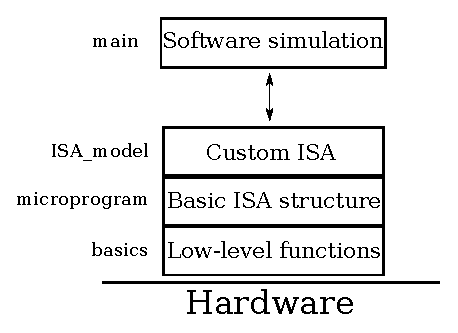
\includegraphics[scale=1]{IMG/structure.eps}
	\caption{Functional structure of the framework.}
	\label{fig:structure}
\end{center}
\end{figure}

In section \ref{sec:arm} we will show how this framework has been implemented and extended
to model the ARMv6-M.

% Alex
\subsection{Functionalities \& possible interpretations}
\label{sec:func}
% Description of the tool-chain and of the ISA design flow
Our main goal with this article is to open the path towards an easier specification and
visualisation of instruction sets. Nonetheless, quite a few other interpretations can be
given to this work. The Domain Specific Language indeed, once that has been used to model
a processor, can be potentially translated into other languages. In turn. they
can be progressively employed with the advantages and tools they come with. It is worth
mentioning that some of the functionalities discussed in this section have not been
implemented yet. Though, they will be part of our future work in this area (see section
\ref{sec:frd}).

The ISA specification might be converted into Event-B language \cite{eventB}. This is a
formal technique used to analyse the model at the system level. It comes with some theorem
provers which are able to verify the consistency of the system, proving that there are 
no inconsistencies between instructions. This is an interesting feature itself, which could
be particularly useful when applied to instruction sets. It falls within the side of the
formal \textit{verification}.

\textit{Visualisation} and \textit{synthesis} are two other
interpretations which can be given to this framework, somehow connected to each other via
CPOG formalism. Even though Haskell provides readable and simple constructs, instruction
set specifications are intrinsically difficult to read and understand by human hand.
Capturing all the dependencies between every micro-operation within the instruction is
complex and, as already mentioned, error-prone. Reading the whole reference manual can take
long. In the light of the above, formal specification can be converted into partial orders,
a visual graph-based representation composed by nodes and arcs, by far more readable either
than reference psuedo-code and Haskell statements.

This allows the user to employ the tool-chain around the conditional partial order
graphs. Either enabling the visual customisation of the dependencies of the instructions in 
\verb|Workcraft|, as well as the usage of the built-in synthesis tools available. A fairly
accurate measurement of the size of the final micro-controller for the processor control
unit can be automatically derived then, allowing the designer to come back at the previous
stage whether some of the requirements (area, power consumption) are not met.

A clearer picture of the whole design-flow can be observed in figure \ref{fig:flow}.

\begin{figure}[ht!]
\begin{center}
	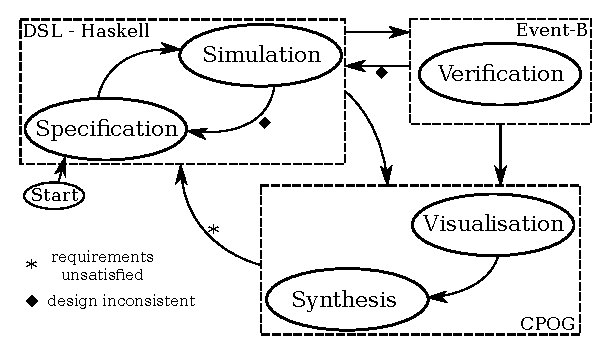
\includegraphics[width=\linewidth]{IMG/flow.eps}
	\caption{Design flow supported by the Haskell-based framework.}
	\label{fig:flow}
\end{center}
\end{figure}

%------------------------------------------------

% Paulius
\section{Case Study}
\label{sec:arm}
% Introduction of ARMv6-M ISA

% Paulius
\subsection{ARMv6-M}
% Description of the model

% Alex & Paulius
\subsection{Towards a readable model}
% Similarities between pseudo reference code and our model
% Show Partial order examples derived by hand
% Maybe an encoding example

%------------------------------------------------

% Alex & Paulius
\section{Conclusion}
\label{sec:conclusion}
% Come up with some interesting conclusions

\subsection{Future research directions}
\label{sec:frd}
% future research direction

\noindent\textbf{Acknowledgements:} The authors would like to thank Dr. Andrey Mokhov for helping with this work.

%------------------------------------------------

\begin{thebibliography}{1}

\bibitem{cpog}
	A. Mokhov, A. Yakovlev. \emph{``Conditional partial order graphs: Model,
	synthesis, and application''}. IEEE Transactions on Computers, Volume 59,
	Pages 1480-1493, November 2010.
	
\bibitem{andreyPhd}
	A. Mokhov. \emph{``Conditional Partial Order Graphs''}. Ph.D. Thesis,
	Newcastle University, September 2009.	

\bibitem{workcraft}
	I. Poliakov, D. Sokolov, A. Mokhov. \emph{``Workcraft: A static data flow
	structure editing, visualisation and analysis tool''}. Petri Nets and Other
	Models of Concurrency - ICATPN 2007. Pages 505-514, 2007.
	
\bibitem{satEncoding}
	A Mokhov, A Alekseyev, A Yakovlev. \emph{``Encoding of processor instruction
	sets with explicit concurrency control''}. Computers \& Digital Techniques,
	IET. Volume 5, Pages 427-439. November 2011.
	
\bibitem{acsd}
	A. de Gennaro, P. Stankaitis, A. Mokhov. \emph{``A Heuristic Algorithm for
	Deriving Compact Models of Processor Instruction Sets''}. 15th International
	Conference on Application of Concurrency to System Design (In Press). June
	24-26, 2015.

\bibitem{armv7}
	A. Fox, M. Myreen. \emph{``A Trustworthy Monadic Formalization of the ARMv7
	Instruction Set Architecture''}. Interactive Theorem Proving (ITP), pages
	243-258, 2010.	
	
\bibitem{isaEventB}
	F. Yuan, K. Eder. \emph{``A Generic Instruction Set Architecture Model in
	Event-B for Early Design Space Exploration''}. Technical Report CSTR-09-006,
	University of Bristol, September 2009.

\bibitem{isaFunc}
	T. A.Cook, E. Harcourt. \emph{``A Functional Specification Language for
	Instruction Set Architectures''}. Proceedings of the 1994 International
	Conference on Computer Languages. Publisher IEEE, pages 11-19. May 1994.
	
\bibitem{isaXml}
	A. Abbas, A. Ahmed, A. Ahmed, W. Uz Zaman Bajwa, A. Anwar, S. Abbasi. 
	\emph{``A retargetable tool-suite for the design of application specific
	instruction set processors using a machine description language''}. IEEE
	International Symposium on Circuits and Systems, 2002. Volume 1, pages 425-428.
	ISCAS 2002.
	
\bibitem{maxPhd}
	M. Rykunov. \emph{``Design of Asynchronous Microprocessor for Power
	Proportionality''}. Ph.D. Thesis, Newcastle University. Technical Report Series
	NCL-EEE-MICRO-TR-2013-182, December 2013.
	
\bibitem{armManual}
	ARM Ltd. \emph{``ARMv6-M Architecture Reference Manual''}. 
	ARM DDI 0419C (ID092410), 2010.
	
\bibitem{haskell}
	----. \emph{``Haskell 98 Language and Libraries The Revised Report''}. 
	Simon Peyton Jones (editor).
	
\bibitem{eventB}
	C. Métayer, J.-R. Abrial, L. Voisin. \emph{``Event-B Language''}. 
	Project IST-511599. $31^{st}$ May 2005
	
\end{thebibliography}

\end{document}